\documentclass[onecolumn, draftclsnofoot,10pt, compsoc]{IEEEtran}
\usepackage{graphicx}
\usepackage{url}
\usepackage{float}
\usepackage{setspace}
\usepackage{caption}


\captionsetup{justification=centering,margin=2cm}
\usepackage{geometry}
\geometry{textheight=9.5in, textwidth=7in}

% 1. Fill in these details
\def \CapstoneTeamName{		Nexusphere}
\def \CapstoneTeamNumber{		48}
\def \GroupMemberOne{			Meghan Mowery}
\def \GroupMemberTwo{			Louis Duvoisin}
\def \GroupMemberThree{			Sarahi Pelayo}
\def \CapstoneProjectName{		A-Frame Live Stream Portal}
\def \CapstoneSponsorCompany{	Oregon State University}
\def \CapstoneSponsorPerson{		Behnam Saeedi}

% 2. Uncomment the appropriate line below so that the document type works
\def \DocType{	%Problem Statement
				%Requirements Document
				%Technology Review
				Design Document
				%Progress Report
				}
			
\newcommand{\NameSigPair}[1]{\par
\makebox[2.75in][r]{#1} \hfil 	\makebox[3.25in]{\makebox[2.25in]{\hrulefill} \hfill		\makebox[.75in]{\hrulefill}}
\par\vspace{-12pt} \textit{\tiny\noindent
\makebox[2.75in]{} \hfil		\makebox[3.25in]{\makebox[2.25in][r]{Signature} \hfill	\makebox[.75in][r]{Date}}}}
% 3. If the document is not to be signed, uncomment the RENEWcommand below
\renewcommand{\NameSigPair}[1]{#1}

%%%%%%%%%%%%%%%%%%%%%%%%%%%%%%%%%%%%%%%
\begin{document}
\begin{titlepage}
    \pagenumbering{gobble}
    \begin{singlespace}
    	\includegraphics[height=4cm]{coe_v_spot1}
        \hfill 
        % 4. If you have a logo, use this includegraphics command to put it on the coversheet.
        %\includegraphics[height=4cm]{CompanyLogo}   
        \par\vspace{.2in}
        \centering
        \scshape{
            \huge CS Capstone \DocType \par
            {\large\today}\par
            \vspace{.5in}
            \textbf{\Huge\CapstoneProjectName}\par
            \vfill
            {\large Prepared for}\par
            \Huge \CapstoneSponsorCompany\par
            \vspace{5pt}
            {\Large\NameSigPair{\CapstoneSponsorPerson}\par}
            {\large Prepared by }\par
            Group\CapstoneTeamNumber\par
            % 5. comment out the line below this one if you do not wish to name your team
            \CapstoneTeamName\par 
            \vspace{5pt}
            {\Large
                \NameSigPair{\GroupMemberOne}\par
                \NameSigPair{\GroupMemberTwo}\par
                \NameSigPair{\GroupMemberThree}\par
            }
            \vspace{20pt}
        }
        \begin{abstract}
        % 6. Fill in your abstract    
        	A-Frame Live Stream Portal is a project that will be used to bring families closer together, even when adversity keeps them apart. 
        	The main parts of this report are the introduction, design viewpoints, and design views.
        \end{abstract}   	 
    \end{singlespace}
\end{titlepage}
\newpage
\pagenumbering{arabic}
\tableofcontents

% 7. uncomment this (if applicable). Consider adding a page break.
\listoffigures
\listoftables
\clearpage

% 8. now you write!
\section{Introduction}
    \subsection{Purpose}
    The purpose of this document is to describe the different physical aspects of this project.
    By describing the aspect of the project in detail, it will be easier to formulate a plan to complete the project.
    This includes describing the design concerns, views, and viewpoints of this project.
    
    \subsection{Scope}
    This document will cover all aspects of the project, including the hardware and software development.
    This document also includes various images related to the system's user interface and design.
    
    \subsection{Context}
    A-frame live stream portal is a project that will utilize various technologies to allow the stakeholder's family to view the stakeholder's wedding live.
    The project consists of three cameras, two regular view and one 360 view which will be live streaming the wedding at 720p and 30fps.
    The project also uses a microphone which will record the audio of the ceremony and will be what the stakeholder's family hears while they are watching the videos.
    Finally, the web portal that will be created will be used by both the stakeholder and the stakeholder's family.
    The stakeholder will have access to an admin page where they can move, add, or delete cameras and microphones as well as change the displayed venue map.
    The users will be able to select any of the available cameras on the map to view the wedding ceremony.
    This way the family of the stakeholder will be able to experience the wedding as if they were there themselves.
    
\begin{thebibliography}{}
\bibitem{IEEEhowto:AFrame}
[online] A-Frame. Available at: https://aframe.io/ [Accessed 2 Nov. 2018].

\bibitem{IEEEhowto:Audio}
Hills, Mark (December 2017). trx: Realtime audio over IP.
[online] Available at: http://www.pogo.org.uk/~mark/trx/
[Accessed 27 Nov. 2018]

\bibitem{IEEEhowto:Microprocessor-video-streaming}
Roberts, L. (2018). Raspberry Pi MJPEG at ~30fps - lewisroberts.com. [online] lewisroberts.com. Available at: https://www.lewisroberts.com/2015/05/15/raspberry-pi-mjpeg-at-30fps/ [Accessed 28 Nov. 2018].
\bibitem{IEEEhowto:ad-hoc}
Pinola, M. (2018). Features and Uses of an Ad Hoc Wireless Network. [online] Lifewire. Available at: https://www.lifewire.com/what-is-an-ad-hoc-wireless-network-2377409 [Accessed 28 Nov. 2018].

\end{thebibliography}

\section{Glossary}
\begin{table}[H]
\caption{Glossary}
\label{tab:Glossary}
\begin{tabular}{ll}
         Access Token/Login Key & Sequence of characters used for authentication \\
         A-Frame & The web framework that will be used for 360 video \\
         CSS & Cascading Style Sheet\\
         Fps & Frames Per Second \\ 
         Jpeg & Joint Photographic Experts Group (image file format) \\ 
         Mbps & Mega bits per second \\
         Mjpeg & Motion Joint Photographic Experts Group
         720p & Progressive video format with 720 horizontal lines\\
         Png & Portable Network Graphics (image file format) \\
         TCP & Transmission Control Protocol\\
         UDP & User Datagram Protocol \\
         USB & Universal Serial Bus\\
         UI & User interface \\
         Server & The computer hosting the website and receiving the video\\ 
         Web Portal & A website that displays information from multiple external sources \\ 
         Wi-fi & Wireless Fidelity
\end{tabular}

\end{table}

\section{Body}

    \subsection{Identified design stakeholders}
    The stakeholders for this project are Behnam and Jenna Saeedi.
    
    \subsection{Identified design concerns}
    This project will require both a user interface (UI) and technological implementation.
    The web portal will have two different interfaces, admin and user, and will be simple and easy to understand.
    The technologies used for this project will be two video cameras, one 360 degree video camera, a microphone, and multiple raspberry pis.
    
    \subsection{Selected design viewpoints}
    %identifies the design concerns to be focused upon within its view and selects the design languages used to record that design view
        \subsubsection{Normal Video}
        The video needs to be live streamed from the wedding to the stakeholder's family.
        This video will ideally stream at 1080p and 30fps with a minimum of 480p, still with 30fps.
        The stream can be interacted with by the stakeholder's family.
        The camera will need to last the entire wedding ceremony.
        Since the camera is a simple portion of this project and does not contain any detailed components the best design language for this system would be a UML use case diagram.
        
        \subsubsection{360 Video}
        The 360 video needs to be live streamed from the wedding to the stakeholder's family.
        This video will ideally stream at 1080p and 30fps, and can be interacted with by the stakeholder's family.
        The camera will need to have a strong enough battery so it can last the entire wedding ceremony.
        Since the camera will be purchased and implemented into the wedding, the best design language for this system would be a UML use case diagram.
        
        \subsubsection{Microprocessor}
        The microprocessor has to have the capability to stream either the regular or 360 degree video to the web portal without any significant delays. 
        
        \subsubsection{Microphone}
        To get the full experience of the wedding for the family of the client along with streaming video there will be audio to accompany it. The system’s design includes three cameras and one microphone. Because the camera streaming is in real time only one audio stream is needed.  
        A subsystem is a camera or microphone connected to a microprocessor. 
        The goal of the microphone is to record and stream audio so it can be projected over the three video broadcasts coming from the subsystems. 
        
        \subsubsection{Web Server Architecture}
        The web server architecture must be designed so all the video and audio streams from the four subsystems can be sent to a web server. 
        The network design must allow for subsystem independence, meaning that if one of the cameras or microphone fails the others must remain unaffected.  
        %probably have images showing how our technologies will be used
        %IE: front end/back end/hardware
        %UI & Video Player/Web Host/Streaming device & Camera
        
        \subsubsection{Desktop UI}
        The user interface needs to be designed in a way that is simple to use for both the client and the end user. 
        A custom website will be designed. The website's UI will be tailored with input from the client.  
        The design will go through a feedback process where a prototype will be presented to the client, and the client will leave feedback as they see fit. 
        After the client's feedback the prototype will be updated and shown to the client again. 
        The web page will require users to login to view the venue map, and be able to select a device from a camera to watch the wedding. 
        Users will also need to be able to return back to the venue map and select a different device. 
        There will also be an admin view from which the client can add, move, and remove cameras, as well as upload a new venue map.
        
        \subsubsection{Mobile UI}
        In addition to working on desktop, the website will also need to be usable on mobile devices. 
        All functionality available in the desktop UI must be available for mobile.
        
    \subsection{Design views}
    %Each view addresses a specific set of design concerns of the stakeholders
        \subsubsection{Normal Video}
        Video in normal view will contain two subsystems consisting of a raspberry pi camera module with a raspberry pi microprocessor. 
        The module with be connected to the raspberry pi's camera port using a ribbon cable. 
        For video streaming, the design will need a video media player. 
        VLC will be used because it has many options to customize the stream so it can meet the requirements of a minimum of 480p with 30fps. 
        The video will be in  MJPEG format and adjusted to a reasonable bit rate at will depend on the strength of the venue's Wi-Fi. 
        
        \subsubsection{360 Video}
        To accommodate the design concerns for the 360 video camera, a camera was chosen that contained all of the specifications that the stakeholder required.
        The purchased camera has live streaming capabilities at at least 1080p and 30 fps as well as a long lifespan.
        To operate the camera, the user will connect it directly to a computer system and operate the camera from the computer.
        The video will then be streamed to the website using A-Frame.
        The team chose to upload the video directly to the website because instead of going through another format such as YouTube or Facebook the stream will directly to the website 
        
        \subsubsection{Microprocessor}
        The raspberry pi microprocessor will be the device used for streaming. 
        It is one of the two parts of each of the four subsystems.
        Three raspberry pis will be streaming video and one raspberry pi will stream audio. 
        The design choices must ensure the system is streaming at a minimum of 720p and 30fps. 
        To get a video stream first a Video For Linux 2 module will be loaded. 
        Next, an open source media player called VLC will be installed onto every camera raspberry pi subsystem and the web server. 
        VLC allows for the use of a command to encode at 30fps and 1080p meeting the system’s video quality requirements however, high quality results in the stream costing 50Mbps.
        VLC has more customization options like changing sharpness and changing bitrate. 
        If 1080p can not be reached, the video stream will be adjusted to 720p or 480p using VLC commands to get a smaller bit rate that will work with the Wi-Fi at the venue. 
        
        \subsubsection{Microphone}
        The best design approach selected will be to have the microphone connected to its own microprocessor.  
        The independence of the mentioned design choices meets the need for safeguarding from total system failure as a result from one competent or subsystem failure. 
        The Mini USB Microphone by Adafruit will be used in unison with a raspberry pi 3 to create the audio subsystem for the project. 
        Because it is for audio, the raspberry pi 3 will have enough power and CPU to process the sound to stream it a decent quality unlike video. 
        The Mini USB microphones has easy interface meaning that it can be inserted into any USB port. 
        Audio will be streamed using UDP and will handle network congestion and dropped packets. 
        Using UDP for audio streaming is more appropriate over TCP streaming per industry standards. 
        Trx is a toolset based on the Linux library ALSA Opus codec lib oRTP for broadcasting live audio. 
        The description of the toolset mentions that the audio can be streamed over public internet therefore it will be streamed over the venues using Wi-Fi. 
        While it is mentioned that streaming over public internet is a security hazard because the toolset does not have a security built into it, that is not a concern of the client therefore not an issue for the project. 
        Commands call for sending audio from one point over IP networks to another point. 
        The raspberry pi will be programmed to capture audio from the Mini USB microphone and sent over Wi-Fi using UPD to the web portal’s server using the server’s IP as the destination. 
        The TXR toolset also has options for customizing the transmitter and receiver parameters to optimize the audio streaming. 
        Examples of some of the options include changing the data rate, changing the size of the buffer, changing the frame size, and jitter buffer to reduce the latency.  
        Using the txr toolset was chosen because it boasts high quality wideband audio with very low latency, as little as a couple milliseconds and very fast recovery from dropped package.
        
        \subsubsection{Web Server Architecture}Each of the microprocessors need to have a built-in wifi module to be able to connect to the internet but most will not need it using an ad hoc network. 
        The network will consists of four subsystems, three video, one audio and a central hub. 
        The raspberry pi in each subsystem will be wirelessly connected to one raspberry pi which will be the central hub.
        The central raspberry pi will be plugged in to the router via ethernet at the venue. 
        The design of an ad hoc network avoids putting to much strain on the microprocessor that might come from independent streaming from each subsystem to the web server.
        By using an ad hoc network the microprocessors in each subsystem can focus on their respective role of video or audio. 
        Each microprocessor will send captured video or audio to the central hub wirelessly. 
        Then the central hub will send the video and audio to the web server over the internet to be served to the web portal.
        The network will be made by setting the raspberry pi 3’s to ad hoc mode. 
        First it is recommended that the original network interfaces be saved as a back up then go in and change the wireless mode. 
        The raspberry pi from a subsystem will have the IP address of the central hub raspberry pi set, a netmask set, a wireless channel will be set, and the wireless mode will be set to ad hoc. 
        These mentioned network interfaces changes will be done for all four of the subsystems to connected the central hub.

        \begin{figure}[H]
            \centering
            \captionsetup{justification=centering,margin=2cm}
            \includegraphics[scale=0.5]{Images/system-architecture.png}
            \centering\caption{System Architecture}
            \label{fig:Architecture}
        \end{figure}
        
        \subsubsection{Desktop UI}
        
        Figure \ref{fig:Login} is a prototype of the UI for the login page of the system's website. Users will be given a login key which they will input. When the user's enter the correct key they will be taken to the main page, Figure \ref{fig:User}. The main page is where users will be able to select which stream they want to watch. The main page also has an admin view shown in Figure \ref{fig:Admin}. The client will be able to get to admin view by logging in with a separate login key for the admin login. The buttons will open menus that will allow the client to perform the labeled action (ex: add a device, remove a device, etc). In both admin and normal user mode clicking on a camera will redirect the user to that camera's stream viewable in Figure \ref{fig:Video}. The video page will be the same for both normal and 360 video.
        
        \begin{figure}[H]
            \centering
            \captionsetup{justification=centering,margin=2cm}
            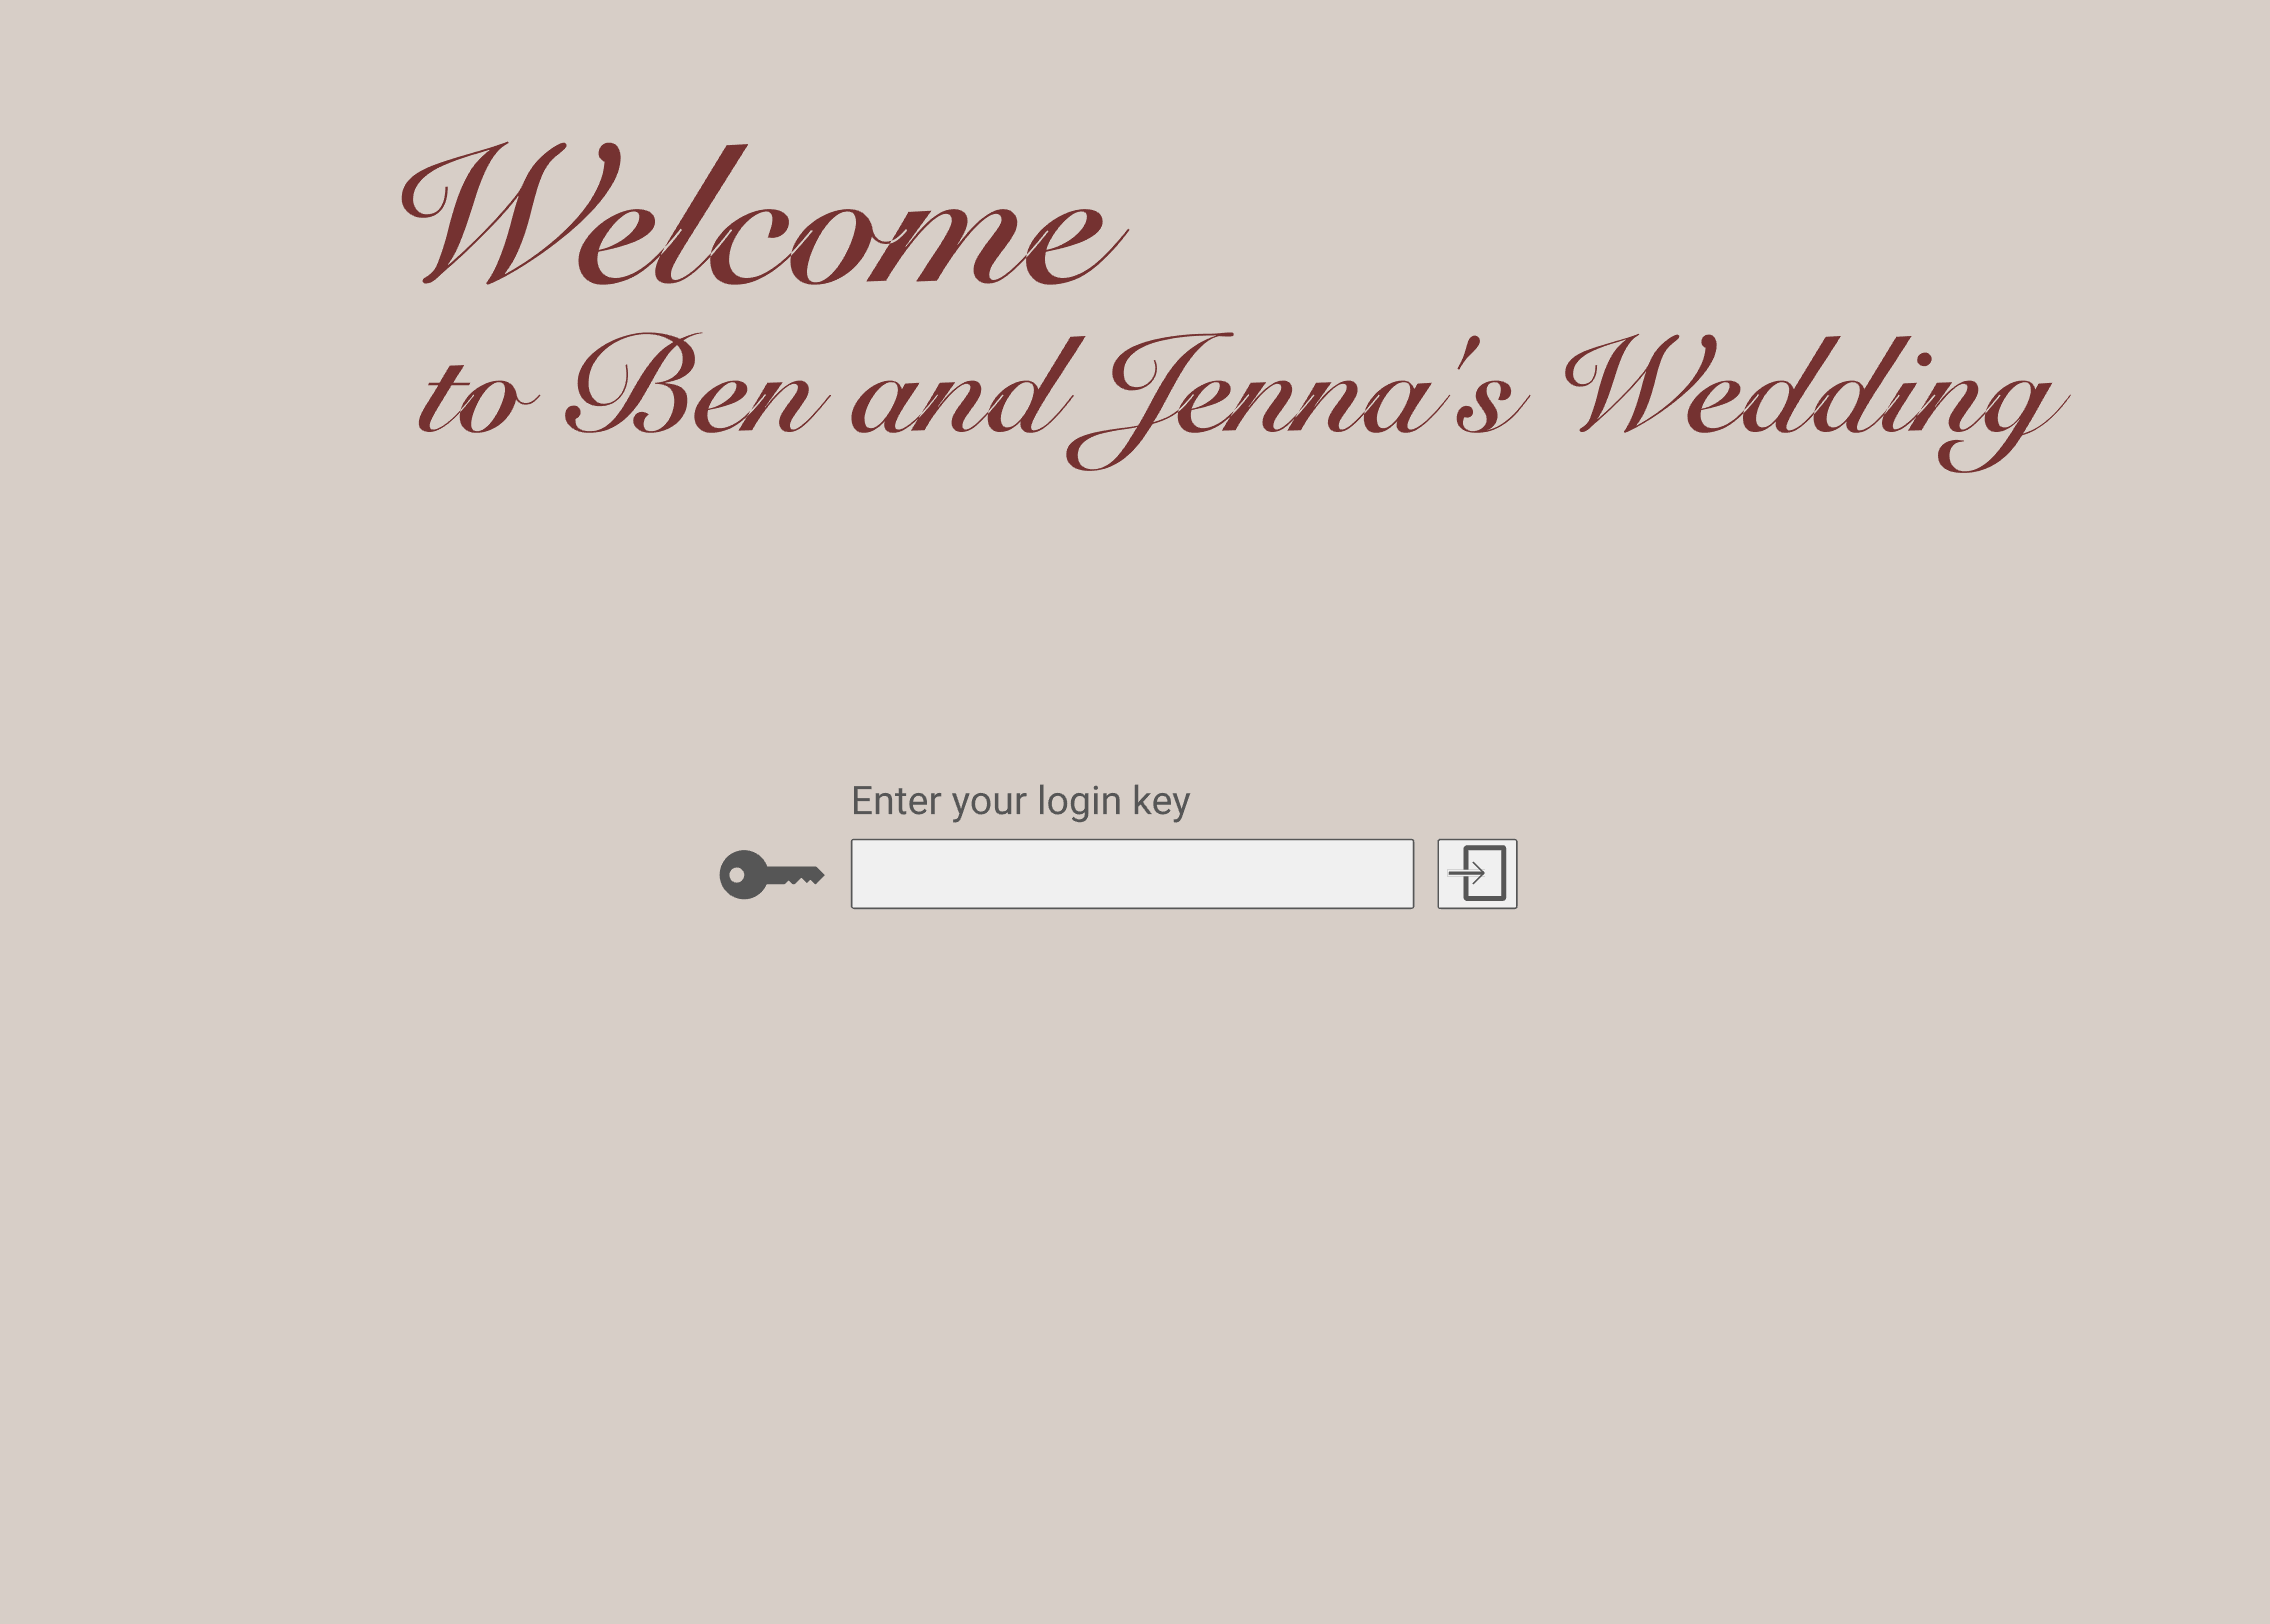
\includegraphics[scale=0.2]{Images/desktop-login.png}
            \centering\caption{Login Page}
            \label{fig:Login}
        \end{figure}
        \begin{figure}[H]
            \centering
            \captionsetup{justification=centering,margin=2cm}
            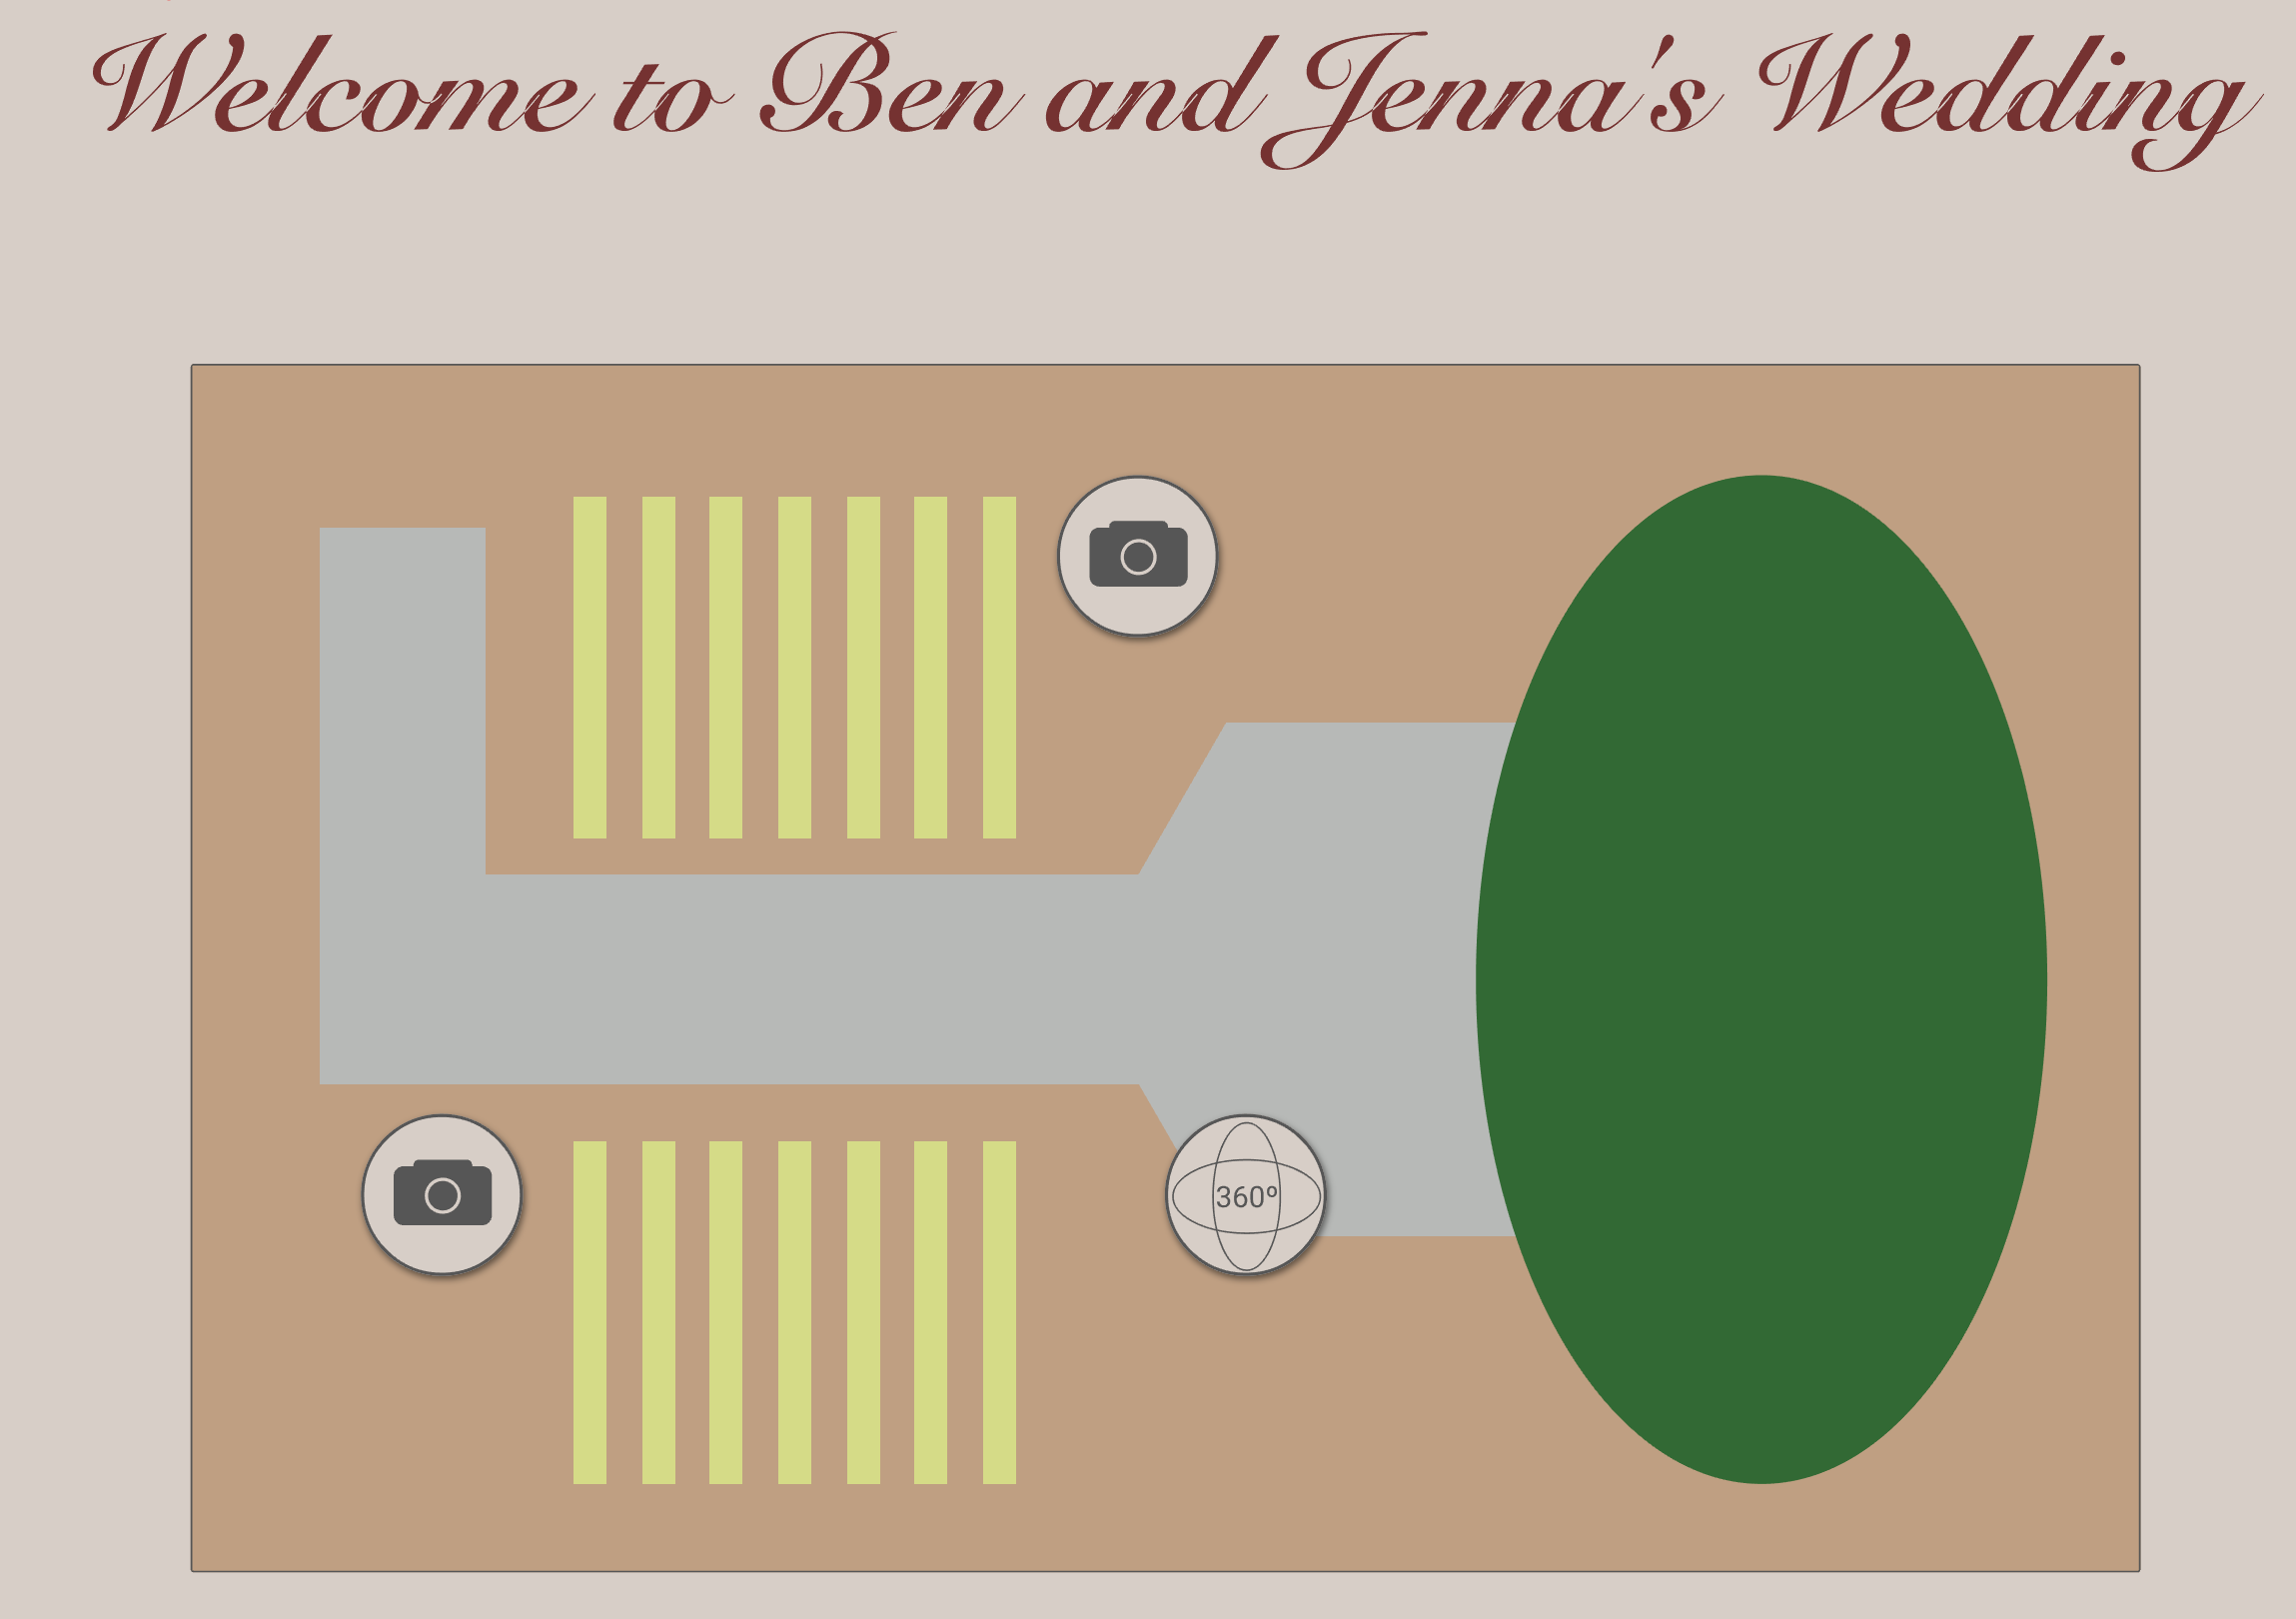
\includegraphics[scale=0.2]{Images/desktop-main.png}
            \centering\caption{User View}
            \label{fig:User}
        \end{figure}
        \begin{figure}[H]
            \centering
            \captionsetup{justification=centering,margin=2cm}
            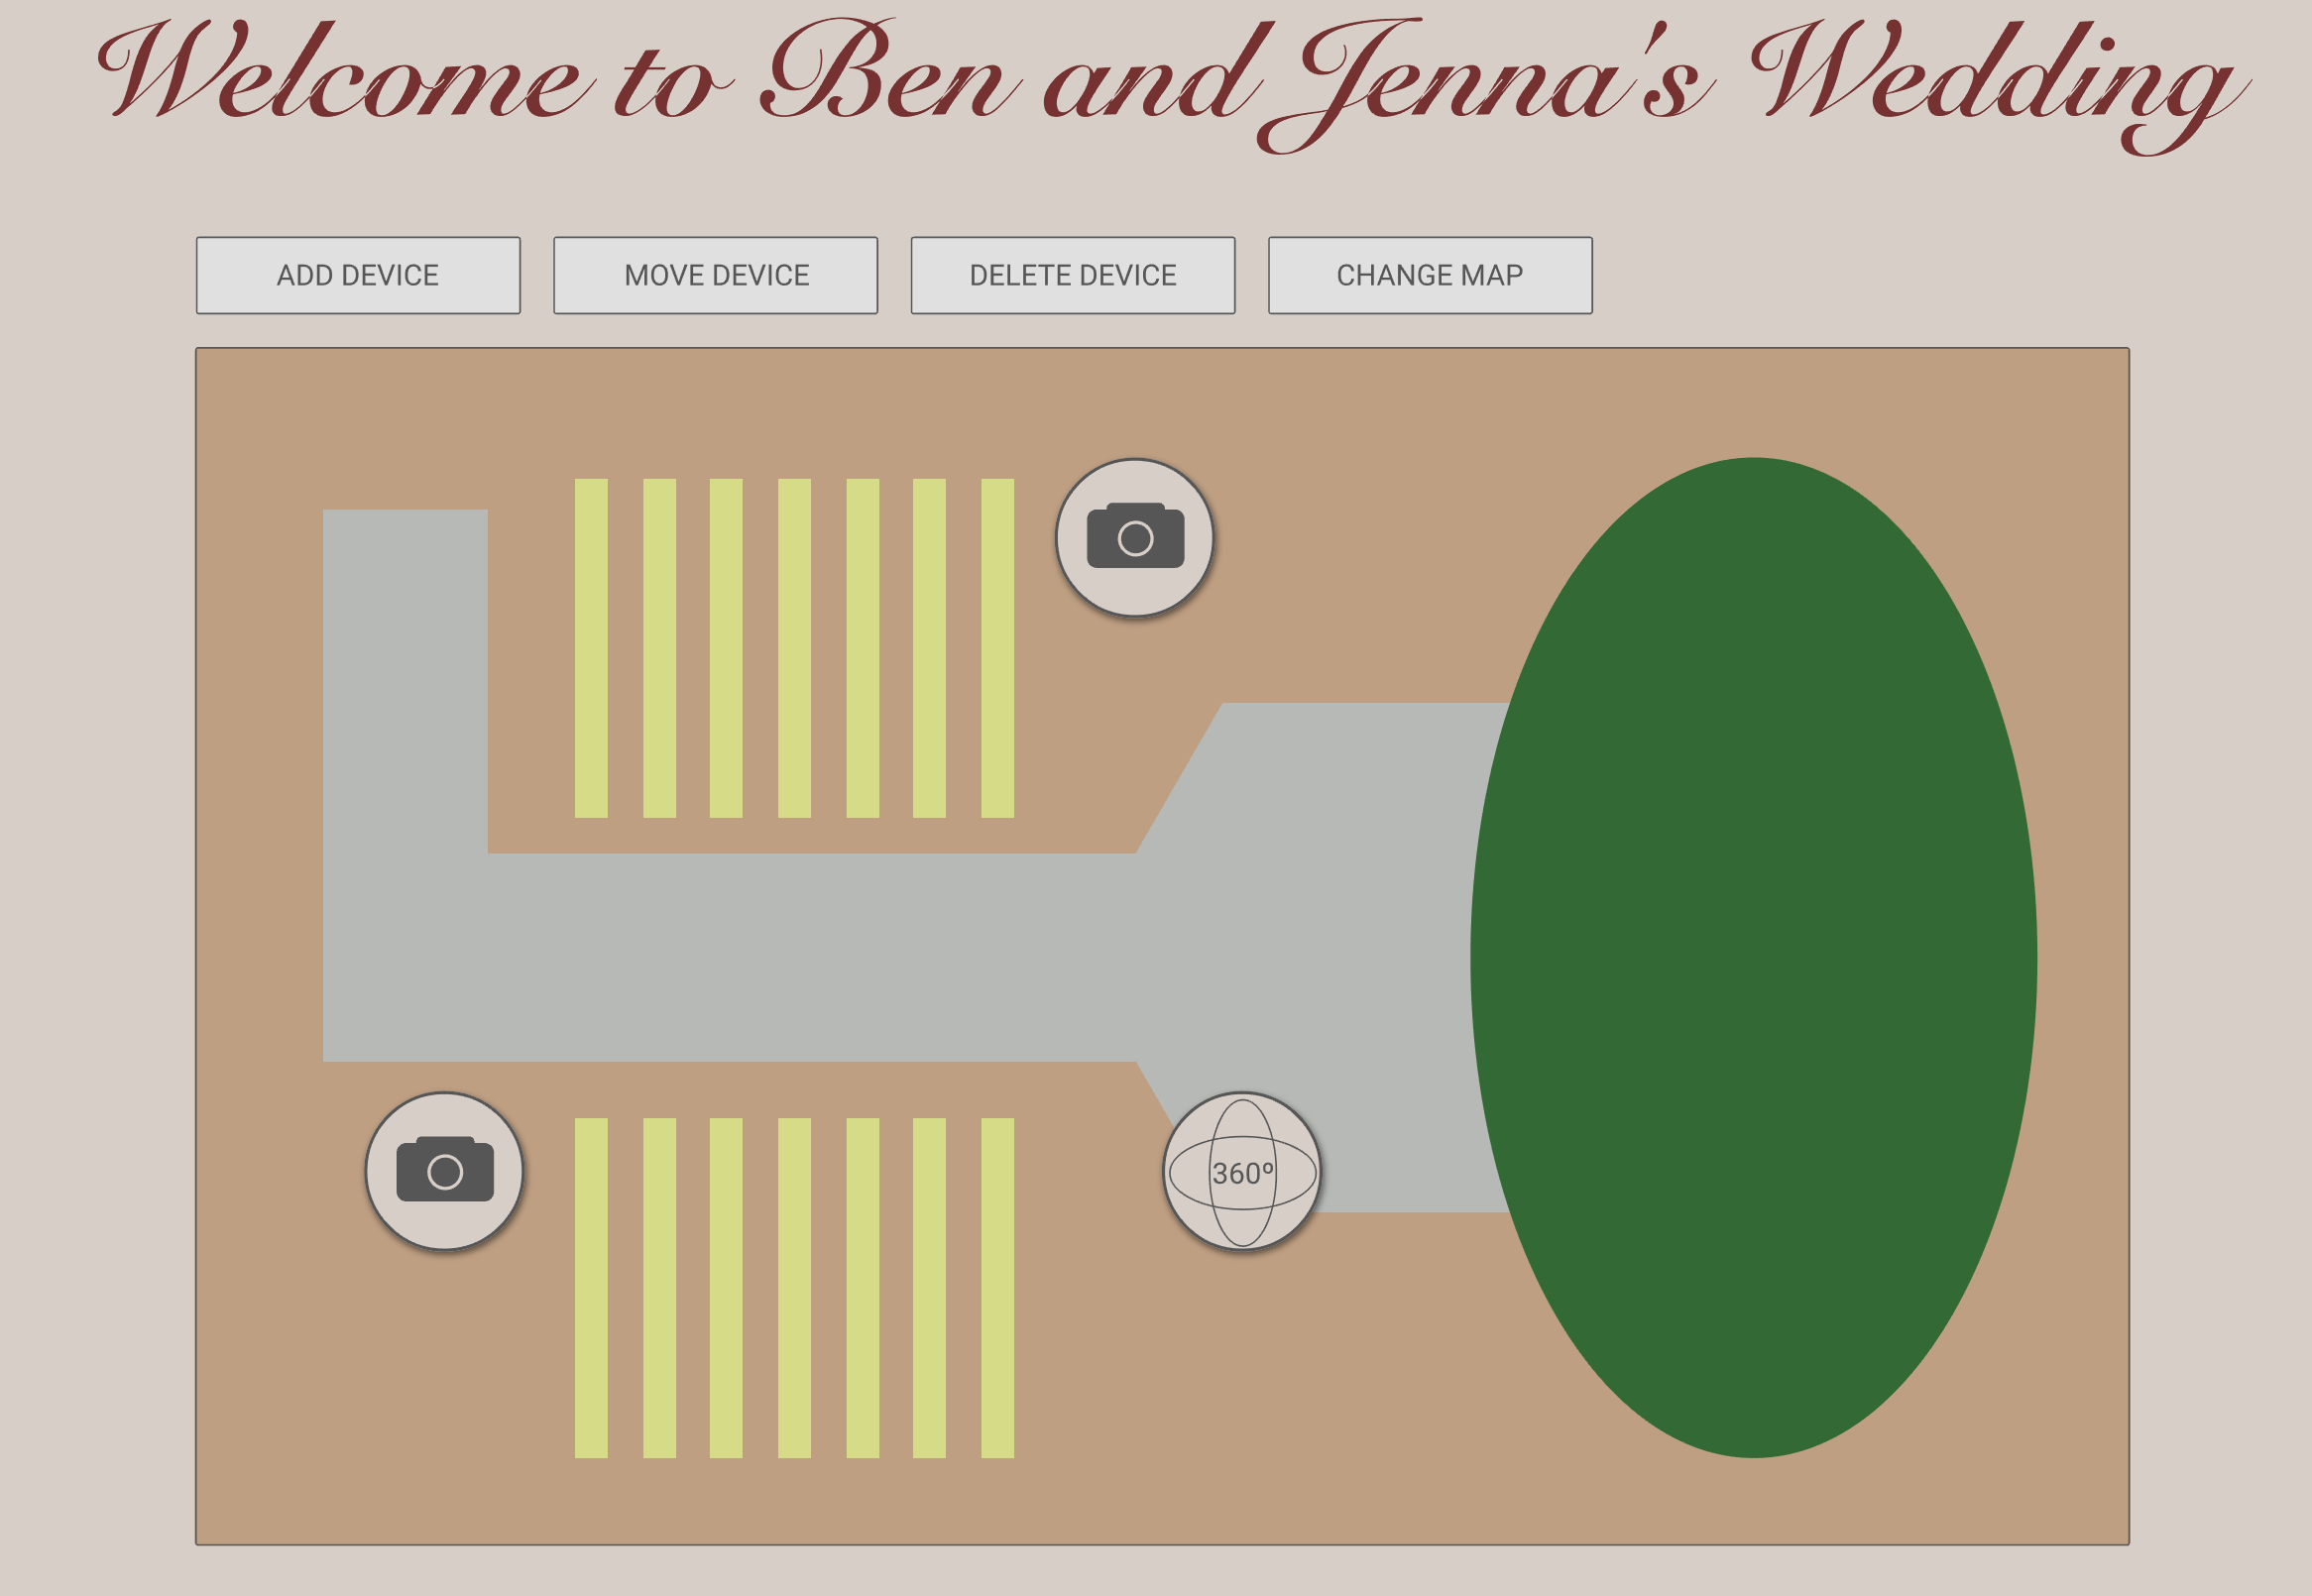
\includegraphics[scale=0.2]{Images/desktop-admin.png}
            \centering\caption{Admin View}
            \label{fig:Admin}
        \end{figure}
        \begin{figure}[H]
            \centering
            \captionsetup{justification=centering,margin=2cm}
            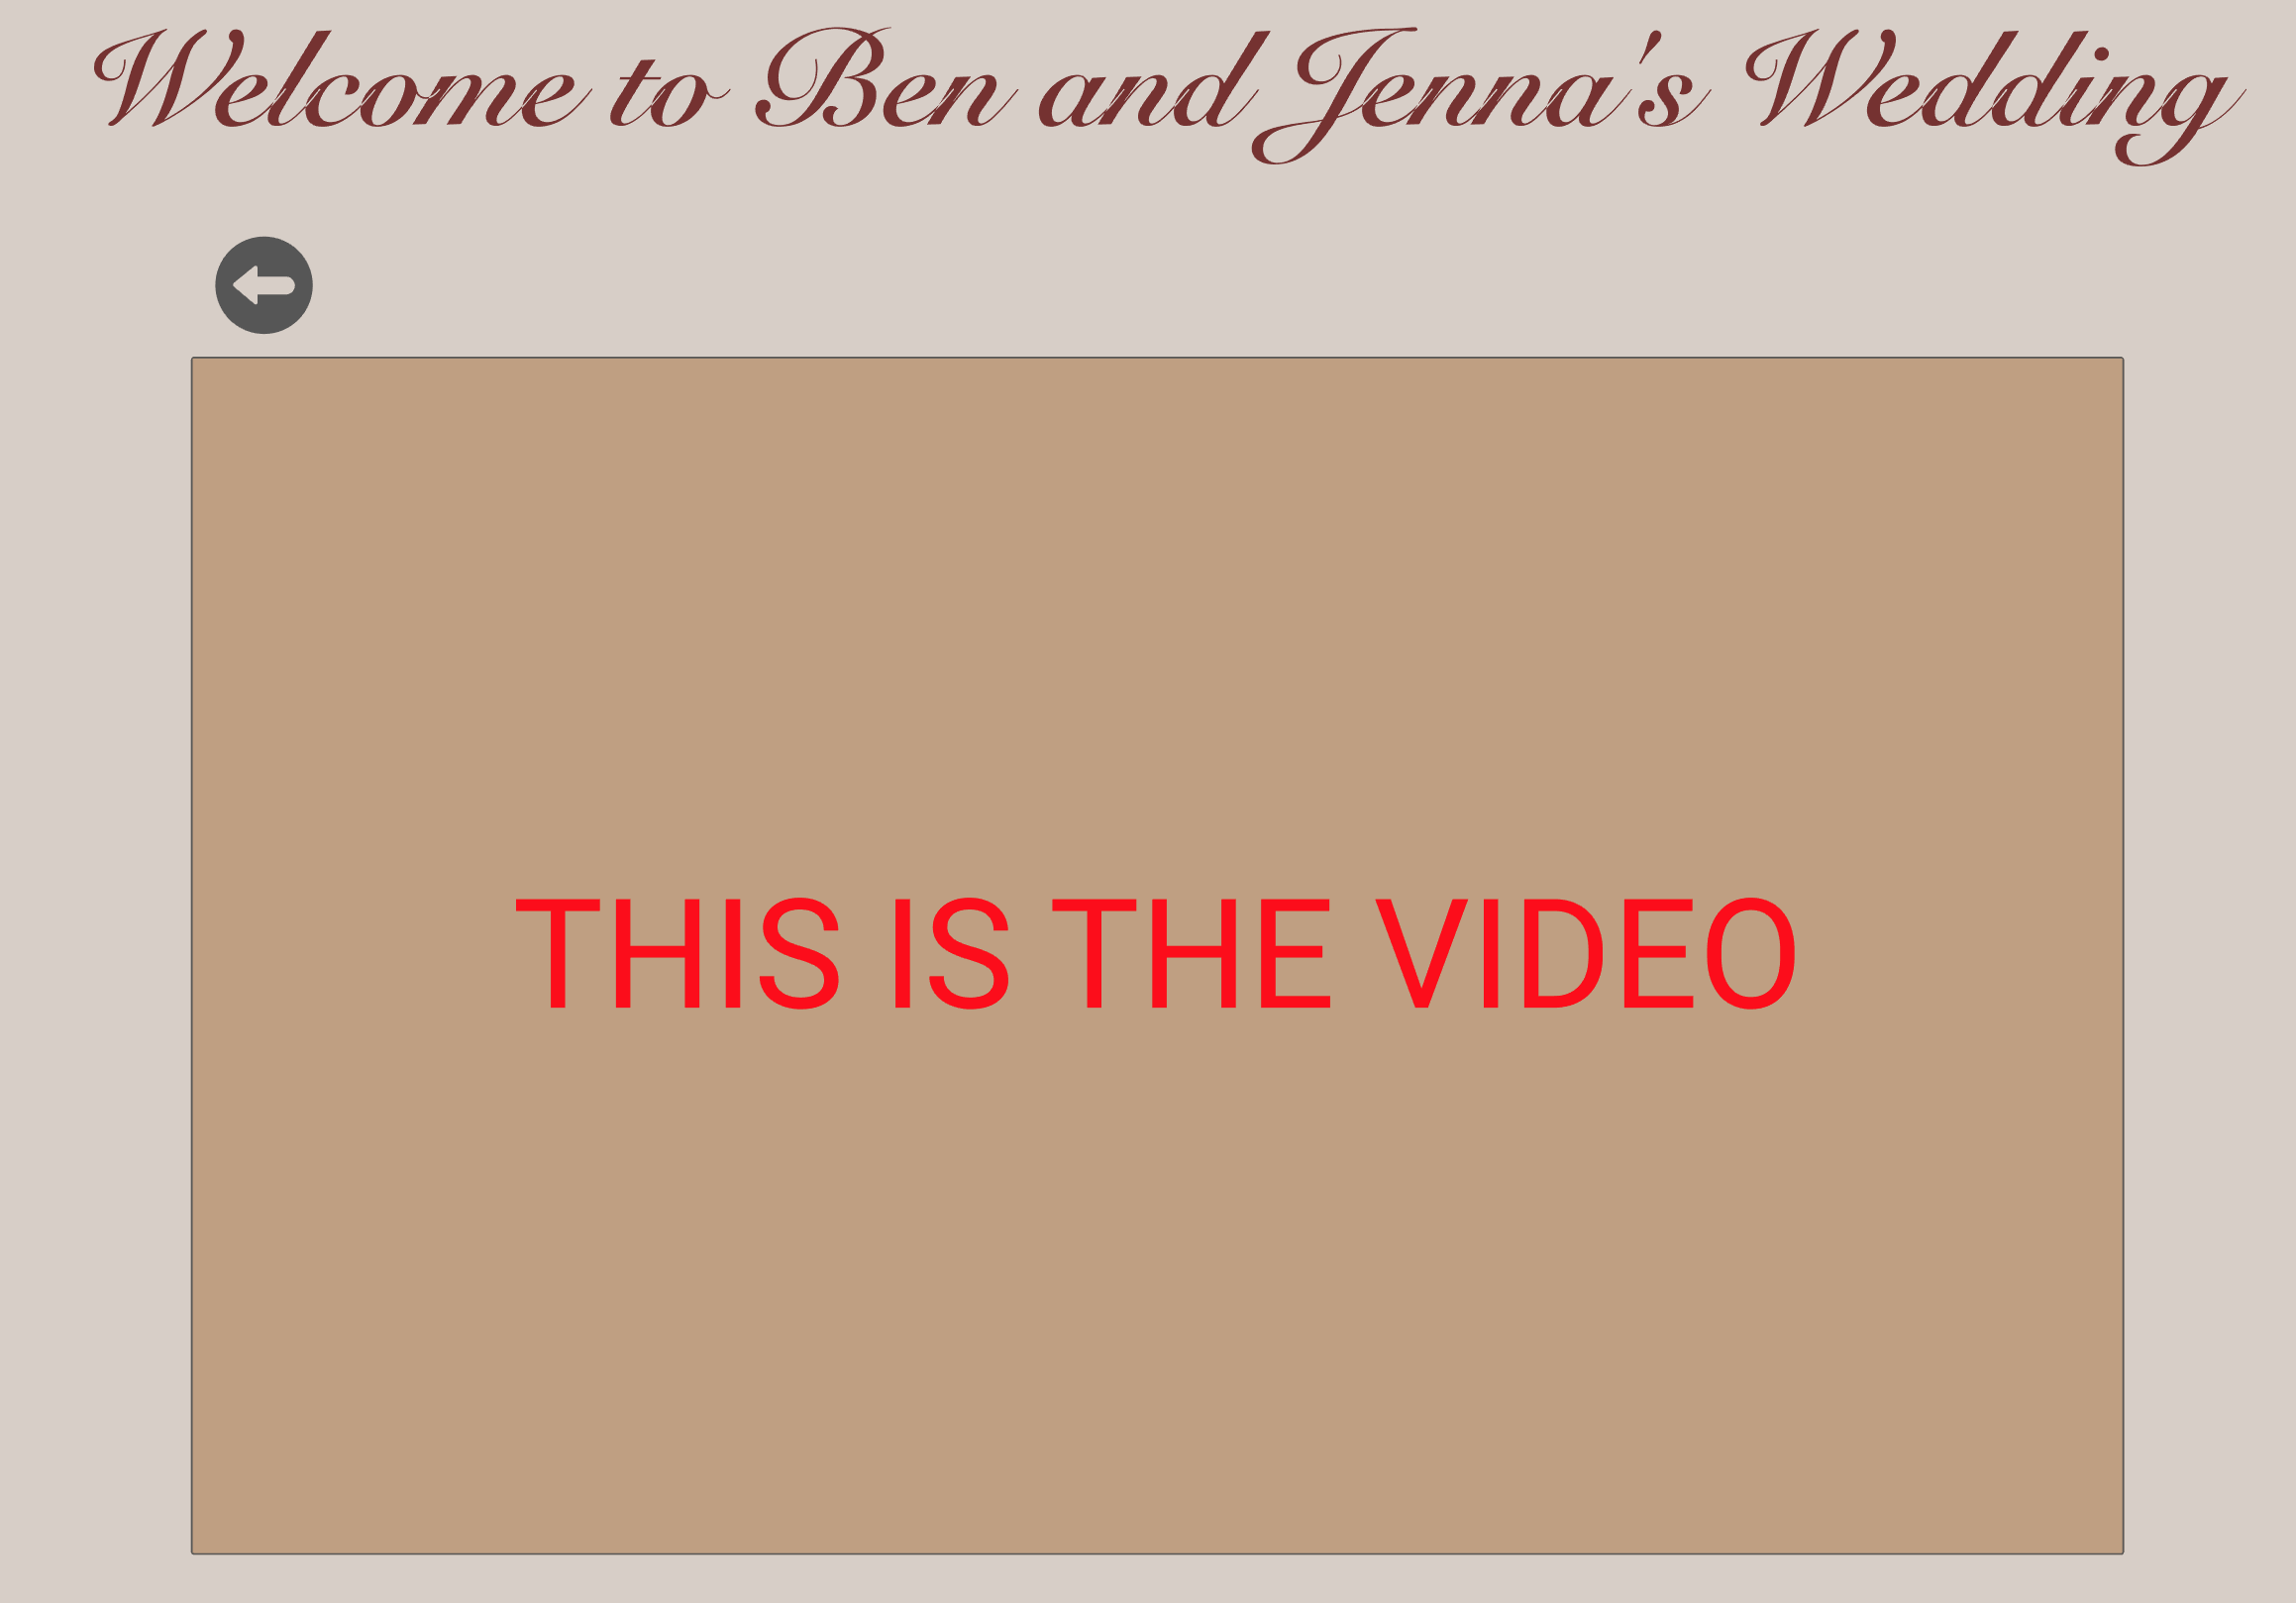
\includegraphics[scale=0.2]{Images/desktop-video.png}
            \centering\caption{Video Page}
            \label{fig:Video}
        \end{figure}
        
        \subsubsection{Mobile UI}
        The mobile UI will contain the same pages as the desktop UI and have all of the same functionality. The system's CSS will be written such that the user will be loading what would be the same page both on desktop and mobile, but the page's components for the mobile view will be oriented differently. 
        
        \begin{figure}[H]
        \minipage{0.45\textwidth}
            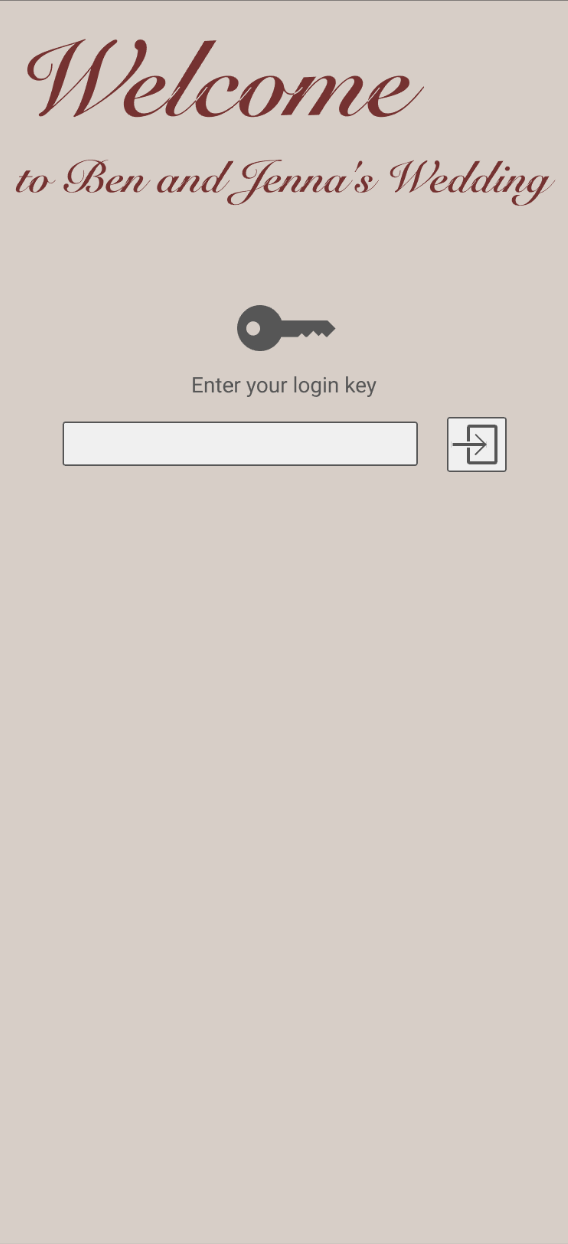
\includegraphics[scale=0.4]{Images/mobile-login.png}
            \centering\caption{Mobile Login Page}
            \label{fig:MLogin}
        \endminipage\hfill
        \minipage{0.45\textwidth}
            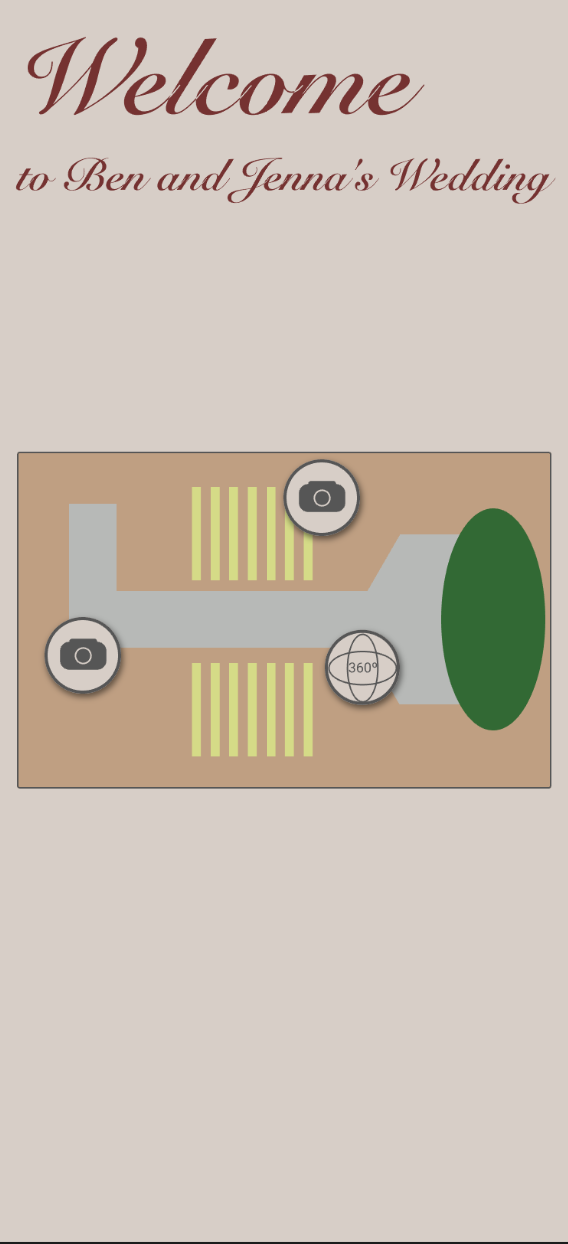
\includegraphics[scale=0.4]{Images/mobile-main.png}
            \centering\caption{Mobile User View}
            \label{fig:MUser}
        \endminipage\hfill

        \end{figure}
         \begin{figure}[H]
         \minipage{0.45\textwidth}
            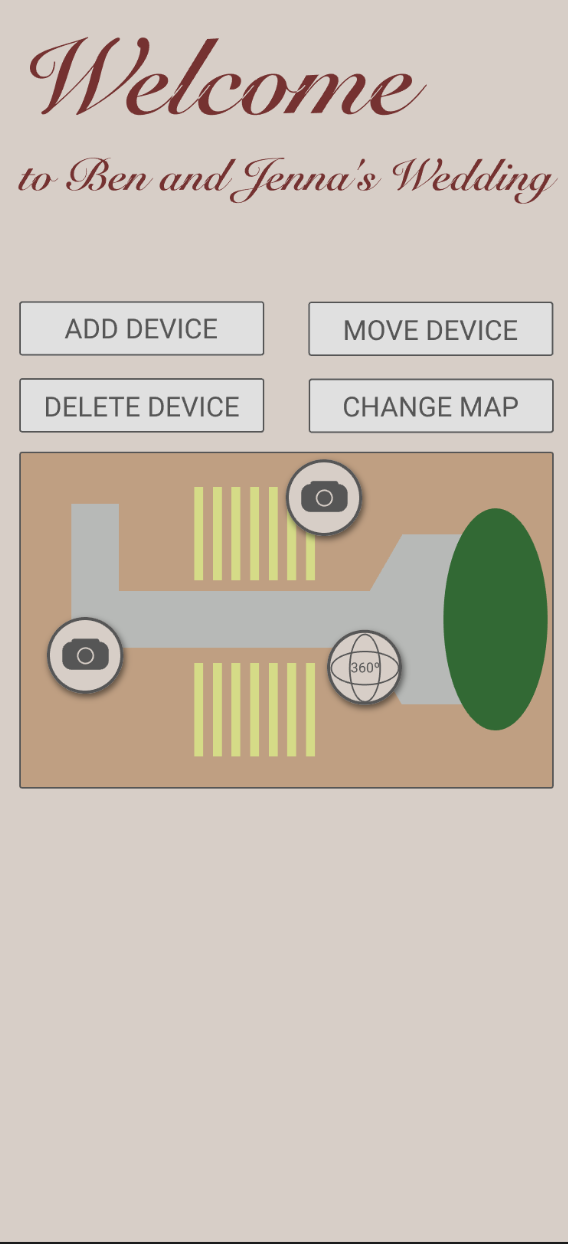
\includegraphics[scale=0.4]{Images/mobile-admin.png}
            \centering\caption{Mobile Admin View}
            \label{fig:MAdmin}
        \endminipage\hfill
        \minipage{0.45\textwidth}
            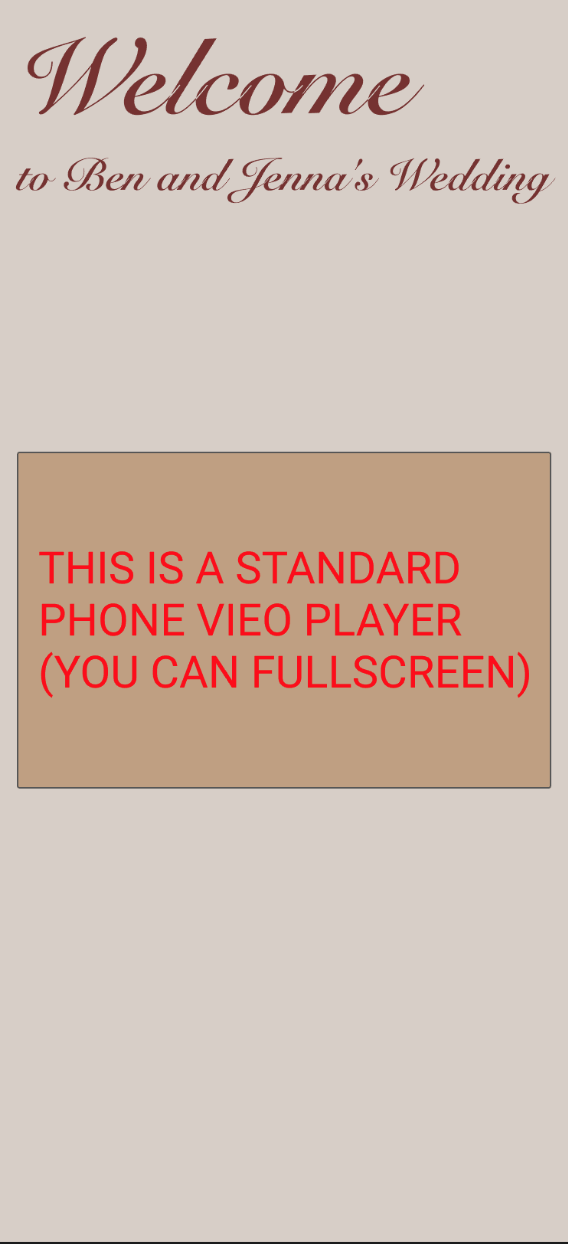
\includegraphics[scale=0.4]{Images/mobile-video.png}
            \centering\caption{Mobile Video Page}
            \label{fig:MVideo}
        \endminipage\hfill
         \end{figure}

\end{document}